\documentclass[aspectratio=169]{beamer}

\mode<presentation>
{
  \usetheme{Warsaw}
  % or ...

  \setbeamercovered{transparent}
  % or whatever (possibly just delete it)
}


\usepackage[english]{babel}
\usepackage[latin1]{inputenc}
\usepackage{graphicx}
%\usepackage{times}
%\usepackage[T1]{fontenc}
% Or whatever. Note that the encoding and the font should match. If T1
% does not look nice, try deleting the line with the fontenc.

\usepackage{amsmath,amsfonts,amssymb}

\newcommand{\pkg}{\textbf}
\newcommand{\code}{\texttt}


\title[The R Language]{Introduction to the R Language}

\subtitle{Functions}

\date{Computing for Data Analysis}

\setbeamertemplate{footline}[page number]


\begin{document}

\begin{frame}
  \titlepage
\end{frame}

\begin{frame}[fragile]{Functions}
Functions are created using the \code{function()} directive and are
stored as R objects just like anything else.  In particular, they are
R objects of class ``function''.
\begin{verbatim}
f <- function(<arguments>) {
        ## Do something interesting
}
\end{verbatim}
Functions in R are ``first class objects'', which means that they can
be treated much like any other R object.  Importantly,
\begin{itemize}
\item
Functions can be passed as arguments to other functions
\item
Functions can be nested, so that you can define a function inside of
another function
\end{itemize}
The return value of a function is the last expression in the function
body to be evaluated.
\end{frame}

\begin{frame}{Function Arguments}
Functions have \textit{named arguments} which potentially have
\textit{default values}.
\begin{itemize}
\item
The \textit{formal arguments} are the arguments included in the
function definition
\item
The \code{formals} function returns a list of all the formal arguments
of a function
\item
Not every function call in R makes use of all the formal arguments
\item
Function arguments can be \textit{missing} or might have default
values
\end{itemize}
\end{frame}

\begin{frame}[fragile]{Argument Matching}
R functions arguments can be matched positionally or by name. So the
following calls to \code{sd} are all equivalent
\begin{verbatim}
> mydata <- rnorm(100)
> sd(mydata)
> sd(x = mydata)
> sd(x = mydata, na.rm = FALSE)
> sd(na.rm = FALSE, x = mydata)
> sd(na.rm = FALSE, mydata)
\end{verbatim}
Even though it's legal, I don't recommend messing around with the
order of the arguments too much, since it can lead to some confusion.
\end{frame}

\begin{frame}[fragile]{Argument Matching}
You can mix positional matching with matching by name.  When an
argument is matched by name, it is ``taken out'' of the argument list
and the remaining unnamed arguments are matched in the order that they
are listed in the function definition.
\begin{verbatim}
> args(lm)
function (formula, data, subset, weights, na.action, 
          method = "qr", model = TRUE, x = FALSE, 
          y = FALSE, qr = TRUE, singular.ok = TRUE, 
          contrasts = NULL, offset, ...) 
\end{verbatim}
The following two calls are equivalent.
\begin{verbatim}
lm(data = mydata, y ~ x, model = FALSE, 1:100)
lm(y ~ x, mydata, 1:100, model = FALSE)
\end{verbatim}
\end{frame}

\begin{frame}{Argument Matching}
\begin{itemize}
\item
Most of the time, named arguments are useful on the command line when
you have a long argument list and you want to use the defaults for
everything except for an argument near the end of the list
\item
Named arguments also help if you can remember the name of the argument
and not its position on the argument list (plotting is a good
example).
\end{itemize}
\end{frame}

\begin{frame}{Argument Matching}
Function arguments can also be \textit{partially} matched, which is
useful for interactive work.  The order of operations when given an
argument is
\begin{enumerate}
\item
Check for exact match for a named argument
\item
Check for a partial match
\item
Check for a positional match
\end{enumerate}
\end{frame}

\begin{frame}[fragile]{Defining a Function}
\begin{verbatim}
f <- function(a, b = 1, c = 2, d = NULL) {
        
}
\end{verbatim}
In addition to not specifying a default value, you can also set an
argument value to \code{NULL}.
\end{frame}

\begin{frame}[fragile]{Lazy Evaluation}
Arguments to functions are evaluated \textit{lazily}, so they are
evaluated only as needed.
\begin{verbatim}
f <- function(a, b) {
        a^2
}
f(2)
\end{verbatim}
This function never actually uses the argument \code{b}, so calling
\code{f(2)} will not produce an error because the 2 gets positionally
matched to \code{a}.  
\end{frame}

\begin{frame}[fragile]{Lazy Evaluation}
Another example
\begin{verbatim}
f <- function(a, b) {
        print(a)
        print(b)
}
\end{verbatim}
\begin{verbatim}
> f(45)
[1] 45
Error in print(b) : argument "b" is missing, with no default
> 
\end{verbatim}
Notice that ``45'' got printed first before the error was triggered.
This is because \code{b} did not have to be evaluated until after
\code{print(a)}.  Once the function tried to evaluate \code{print(b)}
it had to throw an error.
\end{frame}

\begin{frame}[fragile]{The ``...'' Argument}
The \code{...} argument indicate a variable number of arguments that
are usually passed on to other functions.
\begin{itemize}
\item
\code{...} is often used when extending another function and you don't
want to copy the entire argument list of the original function
\begin{verbatim}
myplot <- function(x, y, type = "l", ...) {
        plot(x, y, type = type, ...)
}
\end{verbatim}
\item
Generic functions use \code{...} so that extra arguments can be passed
to methods (more on this later).
\begin{verbatim}
> mean
function (x, ...) 
UseMethod("mean")
\end{verbatim}
\end{itemize}
\end{frame}

\begin{frame}[fragile]{The ``...'' Argument}
The \code{...} argument is also necessary when the number of arguments
passed to the function cannot be known in advance.
\begin{verbatim}
> args(paste)
function (..., sep = " ", collapse = NULL) 

> args(cat)
function (..., file = "", sep = " ", fill = FALSE, 
    labels = NULL, append = FALSE) 
\end{verbatim}
\end{frame}

\begin{frame}[fragile]{Arguments Coming After the ``...'' Argument}
One catch with \code{...} is that any arguments that appear
\textit{after} \code{...} on the argument list must be named
explicitly and cannot be partially matched.
\begin{verbatim}
> args(paste)
function (..., sep = " ", collapse = NULL) 

> paste("a", "b", sep = ":")
[1] "a:b"

> paste("a", "b", se = ":")
[1] "a b :"
\end{verbatim}
\end{frame}


\begin{frame}[fragile]{A Diversion on Binding Values to Symbol}
How does R know which value to assign to which symbol?  When I type
\begin{verbatim}
> lm <- function(x) { x * x }
> lm
function(x) { x * x }
\end{verbatim}
how does R know what value to assign to the symbol \code{lm}?  Why
doesn't it give it the value of \code{lm} that is in the \pkg{stats}
package?
\end{frame}

\begin{frame}[fragile]{A Diversion on Binding Values to Symbol}
When R tries to bind a value to a symbol, it searches through a series
of \code{environments} to find the appropriate value.  When you are
working on the command line and need to retrieve the value of an R
object, the order is roughly
\begin{enumerate}
\item
Search the global environment for a symbol name matching the one
requested.
\item
Search the namespaces of each of the packages on the search list
\end{enumerate}
The search list can be found by using the \code{search} function.
\begin{verbatim}
> search()
[1] ".GlobalEnv"        "package:stats"     "package:graphics" 
[4] "package:grDevices" "package:utils"     "package:datasets" 
[7] "package:methods"   "Autoloads"         "package:base"     
\end{verbatim}
\end{frame}

\begin{frame}[fragile]{Binding Values to Symbol}
\begin{itemize}
\item
The \textit{global environment} or the user's workspace is always the
first element of the search list and the \pkg{base} package is always
the last.  
\item
The order of the packages on the search list matters!
\item
User's can configure which packages get loaded on startup so you
cannot assume that there will be a set list of packages available.
\item
When a user loads a package with \code{library} the namespace of that
package gets put in position 2 of the search list (by default) and
everything else gets shifted down the list.
\item
Note that R has separate namespaces for functions and non-functions so
it's possible to have an object named \code{c} and a function named
\code{c}.
\end{itemize}
\end{frame}

\begin{frame}{Scoping Rules}
The scoping rules for R are the main feature that make it different
from the original S language.  
\begin{itemize}
\item
The scoping rules determine how a value is associated with a free
variable in a function
\item
R uses \textit{lexical scoping} or \textit{static scoping}.  A common
alternative is \textit{dynamic scoping}.
\item
Related to the scoping rules is how R uses the \textit{search list} to
bind a value to a symbol
\item
Lexical scoping turns out to be particularly useful for simplifying
statistical computations
\end{itemize}
\end{frame}

\begin{frame}[fragile]{Lexical Scoping}
Consider the following function.
\begin{verbatim}
f <- function(x, y) {
        x^2 + y / z
}
\end{verbatim}
This function has 2 formal arguments \code{x} and \code{y}.  In the
body of the function there is another symbol \code{z}.  In this case
\code{z} is called a \textit{free variable}.

The scoping rules of a language determine how values are assigned to
free variables.  Free variables are not formal arguments and are not
local variables (assigned insided the function body).
\end{frame}

\begin{frame}[fragile]{Lexical Scoping}
Lexical scoping in R means that
\begin{quote}
\textit{the values of free variables
  are searched for in the environment in which the function was
  defined}.
\end{quote}
What is an environment?
\begin{itemize}
\item
An \textit{environment} is a collection of (symbol, value) pairs,
i.e. \code{x} is a symbol and \code{3.14} might be its value.
\item
Every environment has a parent environment; it is possible for an
environment to have multiple ``children''
\item
the only environment without a parent is the empty environment
\item
A function + an environment = a \textit{closure} or \textit{function
  closure}.
\end{itemize}
\end{frame}


\begin{frame}{Lexical Scoping}
Searching for the value for a free variable:
\begin{itemize}
\item
If the value of a symbol is not found in the environment in which a
function was defined, then the search is continued in the
\textit{parent environment}.
\item
The search continues down the sequence of parent environments until we
hit the \textit{top-level environment}; this usually the global
environment (workspace) or the namespace of a package.
\item
After the top-level environment, the search continues down the search
list until we hit the \textit{empty environment}.
\item
If a value for a given symbol cannot be found once the empty
environment is arrived at, then an error is thrown.
\end{itemize}
\end{frame}


\begin{frame}{Lexical Scoping}
Why does all this matter?
\begin{itemize}
\item
Typically, a function is defined in the global environment, so that
the values of free variables are just found in the user's workspace
\item
This behavior is logical for most people and is usually the ``right
thing'' to do
\item
However, in R you can have functions defined \textit{inside other
  functions}
\begin{itemize}
\item
Languages like C don't let you do this
\end{itemize}
\item
Now things get interesting --- In this case the environment in which a
function is defined is the body of another function!
\end{itemize}
\end{frame}

\begin{frame}[fragile]{Lexical Scoping}
\begin{verbatim}
make.power <- function(n) {
        pow <- function(x) {
                x^n
        }
        pow
}
\end{verbatim}
This function returns another function as its value.
\begin{verbatim}
> cube <- make.power(3)
> square <- make.power(2)
> cube(3)
[1] 27
> square(3)
[1] 9
\end{verbatim}
\end{frame}

\begin{frame}[fragile]{Exploring a Function Closure}
What's in a function's environment?
\begin{verbatim}
> ls(environment(cube))
[1] "n"   "pow"
> get("n", environment(cube))
[1] 3

> ls(environment(square))
[1] "n"   "pow"
> get("n", environment(square))
[1] 2
\end{verbatim}
\end{frame}

\begin{frame}[fragile]{Lexical vs. Dynamic Scoping}
\begin{verbatim}
y <- 10

f <- function(x) {
        y <- 2
        y^2 + g(x)
}

g <- function(x) {
        x * y
}
\end{verbatim}
What is the value of
\begin{verbatim}
f(3)
\end{verbatim}
\end{frame}

\begin{frame}[fragile]{Lexical vs. Dynamic Scoping}
\begin{itemize}
\item
With lexical scoping the value of \code{y} in the function \code{g} is
looked up in the environment in which the function was defined, in
this case the global environment, so the value of \code{y} is 10.
\item
With dynamic scoping, the value of \code{y} is looked up in the
environment from which the function was \textit{called} (sometimes
referred to as the \textit{calling environment}).
\begin{itemize}
\item
In R the calling environment is known as the \textit{parent frame}
\end{itemize}
So the value of \code{y} would be 2.
\end{itemize}
\end{frame}

\begin{frame}[fragile]{Lexical vs. Dynamic Scoping}
When a function is \textit{defined} in the global environment and is
subsequently \textit{called} from the global environment, then the
defining environment and the calling environment are the same.  This
can sometimes give the appearance of dynamic scoping.
\begin{verbatim}
> g <- function(x) {
+         a <- 3
+         x + a + y
+ }
> g(2)
Error in g(2) : object "y" not found
> y <- 3
> g(2)
[1] 8
\end{verbatim}
\end{frame}


\begin{frame}{Other Languages}
Other languages that support lexical scoping
\begin{itemize}
\item
Scheme
\item
Perl
\item
Python
\item
Common Lisp (all languages converge to Lisp)
\end{itemize}
\end{frame}

\begin{frame}{Consequences of Lexical Scoping}
\begin{itemize}
\item
In R, all objects must be stored in memory
\item
All functions must carry a pointer to their respective defining
environments, which could be anywhere
\item
In S-PLUS, free variables are always looked up in the global
workspace, so everything can be stored on the disk because the
``defining environment'' of all functions is the same.
\end{itemize}
\end{frame}

\begin{frame}{Application: Optimization}
Why is any of this information useful?
\begin{itemize}
\item
Optimization routines in R like \code{optim}, \code{nlm}, and
\code{optimize} require you to pass a function whose argument is a
vector of parameters (e.g. a log-likelihood)
\item
However, an object function might depend on a host of other things
besides its parameters (like \textit{data})
\item
When writing software which does optimization, it may be desirable to
allow the user to hold certain parameters fixed
\end{itemize}
\end{frame}

\begin{frame}[fragile]{Maximizing a Normal Likelihood}
Write a ``constructor'' function
\begin{verbatim}
make.NegLogLik <- function(data, fixed=c(FALSE,FALSE)) {
        params <- fixed
        function(p) {
                params[!fixed] <- p
                mu <- params[1]
                sigma <- params[2]
                a <- -0.5*length(data)*log(2*pi*sigma^2)
                b <- -0.5*sum((data-mu)^2) / (sigma^2)
                -(a + b)
        }
}
\end{verbatim}
\textbf{Note}: Optimization functions in R \textit{minimize}
functions, so you need to use the negative log-likelihood.
\end{frame}


\begin{frame}[fragile]{Maximizing a Normal Likelihood}
\begin{verbatim}
> set.seed(1); normals <- rnorm(100, 1, 2)
> nLL <- make.NegLogLik(normals)
> nLL
function(p) {
                params[!fixed] <- p
                mu <- params[1]
                sigma <- params[2]
                a <- -0.5*length(data)*log(2*pi*sigma^2)
                b <- -0.5*sum((data-mu)^2) / (sigma^2)
                -(a + b)
        }
<environment: 0x165b1a4>
> ls(environment(nLL))
[1] "data"   "fixed"  "params"
\end{verbatim}
\end{frame}

\begin{frame}[fragile]{Estimating Parameters}
\begin{verbatim}
> optim(c(mu = 0, sigma = 1), nLL)$par
      mu    sigma 
1.218239 1.787343 
\end{verbatim}
Fixing $\sigma = 2$
\begin{verbatim}
> nLL <- make.NegLogLik(normals, c(FALSE, 2))
> optimize(nLL, c(-1, 3))$minimum
[1] 1.217775
\end{verbatim}
Fixing $\mu = 1$
\begin{verbatim}
> nLL <- make.NegLogLik(normals, c(1, FALSE))
> optimize(nLL, c(1e-6, 10))$minimum
[1] 1.800596
\end{verbatim}
\end{frame}

\begin{frame}[fragile]{Plotting the Likelihood}
\begin{verbatim}
nLL <- make.NegLogLik(normals, c(1, FALSE))
x <- seq(1.7, 1.9, len = 100)
y <- sapply(x, nLL)
plot(x, exp(-(y - min(y))), type = "l")

nLL <- make.NegLogLik(normals, c(FALSE, 2))
x <- seq(0.5, 1.5, len = 100)
y <- sapply(x, nLL)
plot(x, exp(-(y - min(y))), type = "l")
\end{verbatim}
\end{frame}


\begin{frame}{Plotting the Likelihood}
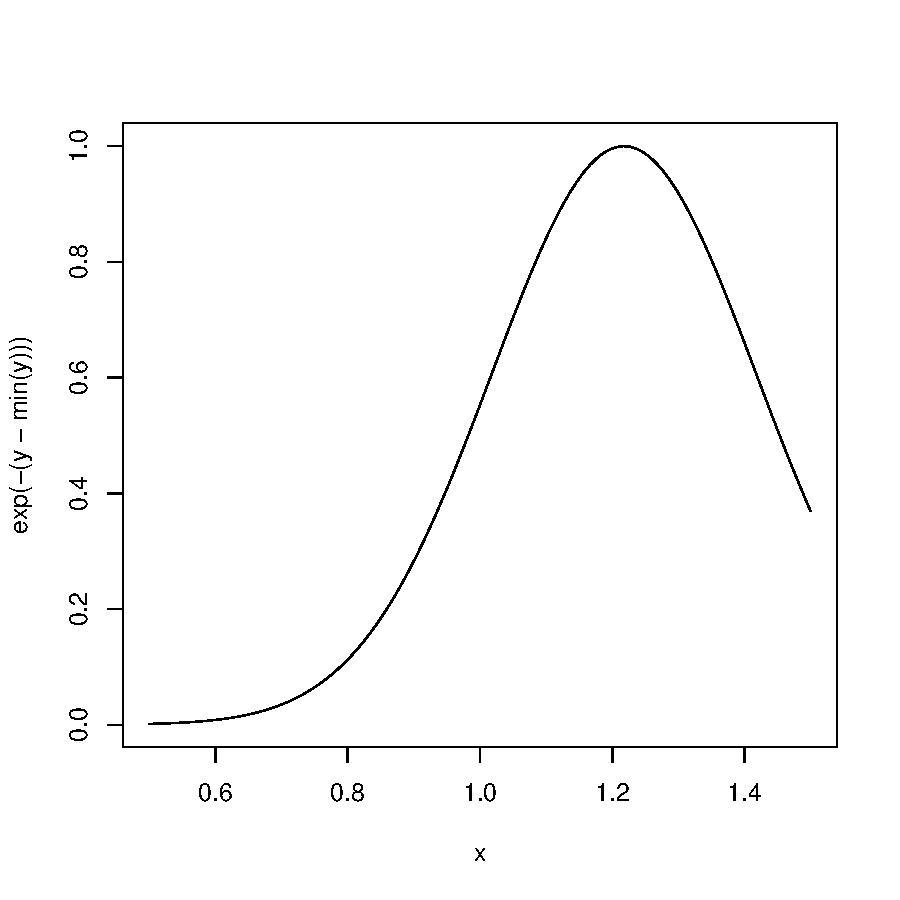
\includegraphics[width=3in,height=3in]{mulike}
\end{frame}

\begin{frame}{Plotting the Likelihood}
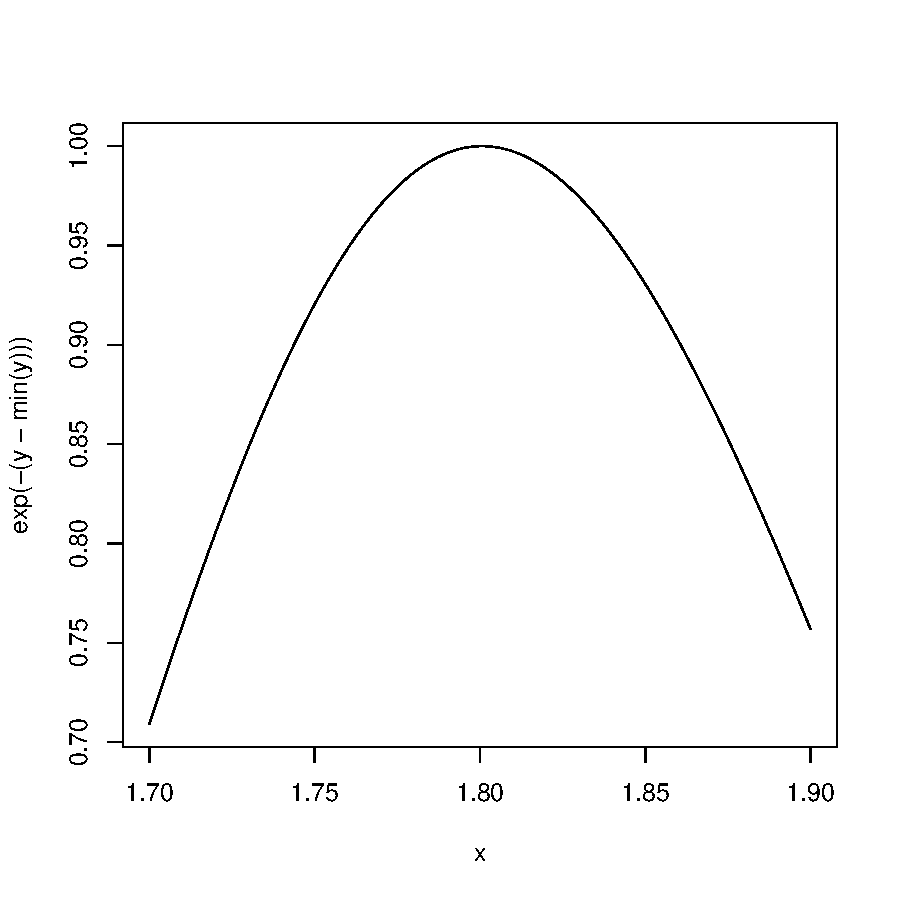
\includegraphics[width=3in,height=3in]{sigmalike}
\end{frame}


\begin{frame}{Lexical Scoping Summary}
\begin{itemize}
\item
Objective functions can be ``built'' which contain all of the
necessary data for evaluating the function
\item
No need to carry around long argument lists --- useful for interactive
and exploratory work.
\item
Code can be simplified and cleand up
\item
Reference: Robert Gentleman and Ross Ihaka (2000). ``Lexical Scope and
Statistical Computing,'' \textit{JCGS}, 9, 491--508.
\end{itemize}
\end{frame}



\end{document}
